\chapter{ارسال رایانامه با اِگزیم 
    \lr{«Exim»}
    }
یاین ابزار گرافیکی برای مدیریت بانک‌های اطلاعاتی مای‌اس‌کیوال در اکثربرخی مواقع پیش‌می‌آید که می‌خواهیم توسط سرور واقعی و یا سند‌باکس برخی پیغام‌ها و اطلاعات را به رایانامه خود و یا دیگران ارسال کنید، برای این کار باید یک سرور رایانامه برای مدیریت رایانامه خود ایجاد کنید. برای این‌کار ابزار متن‌باز و آزادی با نام اگزیم وجود دارد که به راحتی از مخازن اوبونتو قابل نصب است. این ابزار یک سرور رایانامه سبک و ساده است که برای کاربرد فعلی ما بسیار مناسب به نظر می‌رسد.

در این نرم‌افزار ما رایانامه جی‌میل «GMail» یا دیگر رایانامه‌های دارای قابلیت اتصال اس‌ام‌تی‌پی «SMTP» را به آن می‌افزاییم و ابزار بالا با استفاده از رایانامه درج شده، برای رایانه‌های دیگر رایانامه‌های متنوعی را ارسال خواهد کرد. برای نصب نرم‌افزار بالا دستور زیر را اجرا می‌کنیم تا با استفاده از ای‌پی‌تی بسته‌نرم‌افزاری مورد نظر بارگیری و نصب شود.
\newline
\begin{latin}  
    \lstinputlisting[numbers=right,language=SH, framexleftmargin=5mm, frame=shadowbox,rulesepcolor=\color{Black}]{Code/exin-install.sh}
\end{latin}
حال باید با استفاده از دستور «dpkg» به تنظیم این نرم‌افزار بپردازیم. برای این‌کار دستور زیر را اجرا کنید.
تمامی مراحل نمایش داده شده را طبق تصاویر زیر به پیش ببرید، یعنی برای پیغام اول گزینه دوم را انتخاب کنید و  گزینه‌های گفته شده را مطابق تصاویر انتخاب کنید تا الی آخر که  همان‌طور که مشاهده می‌کنید، تمامی موارد در تصاویر مشخص شده‌است. \ref{MAIL-SERVER-EXIM}
\begin{figure}
    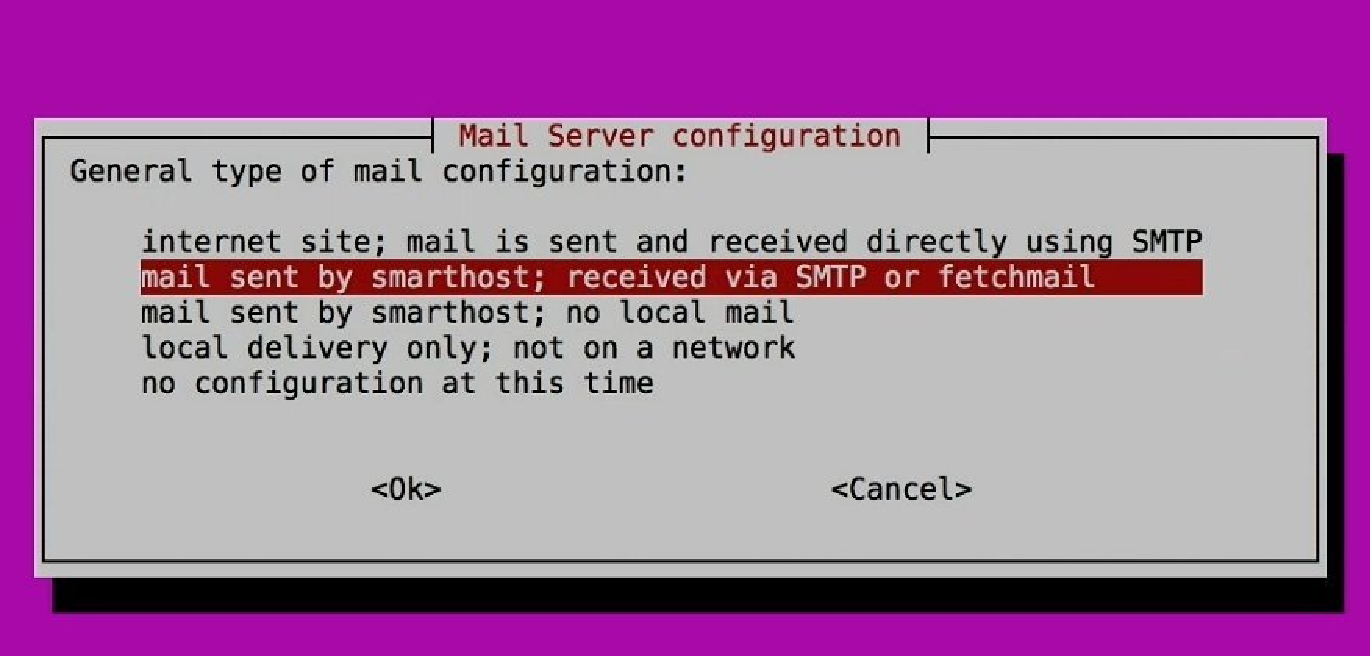
\includegraphics[width=.9\textwidth ,height=.45\textwidth]{Pic/EXIM1}
    \caption{ تنظیمات نرمافزار 
        \lr{ Exim}   
    }
    \label{MAIL-SERVER-EXIM}
\end{figure}
در مرحله بعدی نامی را به دلخواه وارد می‌کنیم. در این مرحله ما همان نام پیش‌فرض را در نظر گرفته‌ایم. \ref{MAIL-SERVER-EXIM2}
\begin{figure}
    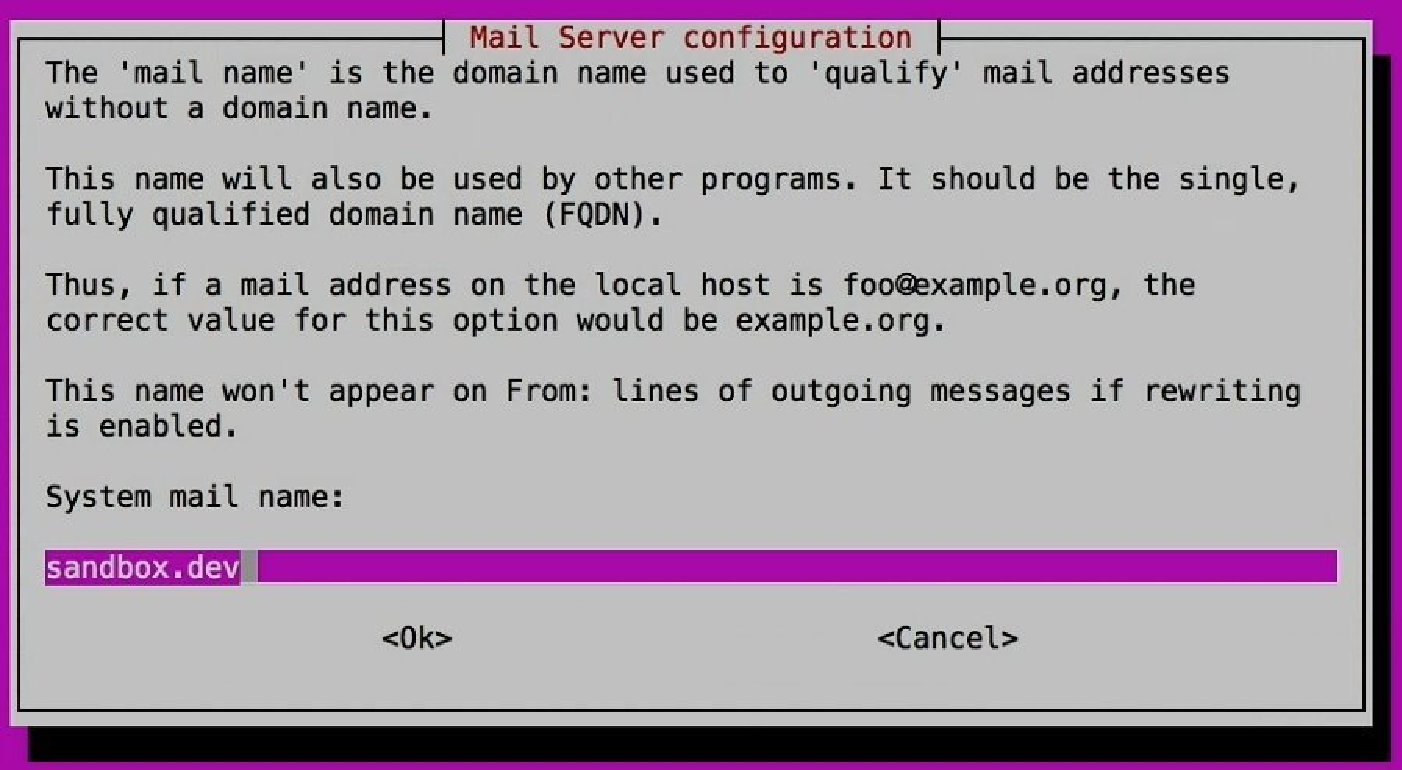
\includegraphics[width=.9\textwidth ,height=.45\textwidth]{Pic/EXIM2}
    \caption{ تنظیمات نرمافزار 
        \lr{ Exim}
        \lr{"Host Name"}   
    }
    \label{MAIL-SERVER-EXIM2}
\end{figure}
سپس در مرحله بعدی بر روی دکمه OK کلیک می‌کنیم تا وارد مرحله بعدی شویم. \ref{MAIL-SERVER-EXIM3}
\begin{figure}
    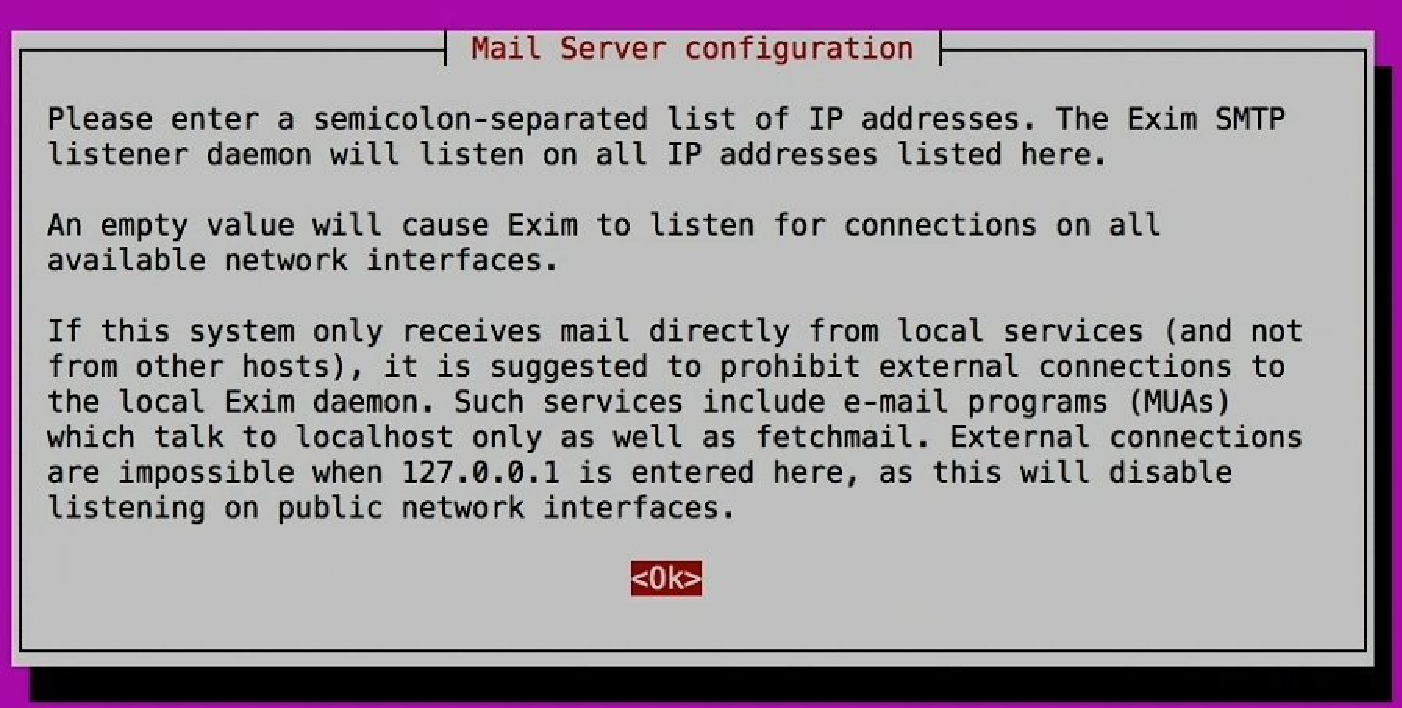
\includegraphics[width=.9\textwidth ,height=.45\textwidth]{Pic/EXIM3}
    \caption{ تنظیمات نرمافزار 
        \lr{ Exim}
        \lr{"Confirm"}   
    }
    \label{MAIL-SERVER-EXIM3}
\end{figure}
سپس کادر بعدی را نیز بدون تغییر مقدار پیش‌فرض، رها می‌کنیم سپس بر روی دکمه تایید کلید اینتر را فشار داده و کادر محاوره‌ای مرحله بعدی را نیز بدون تغییر تایید می‌کنیم. \ref{MAIL-SERVER-EXIM4}
\begin{figure}
    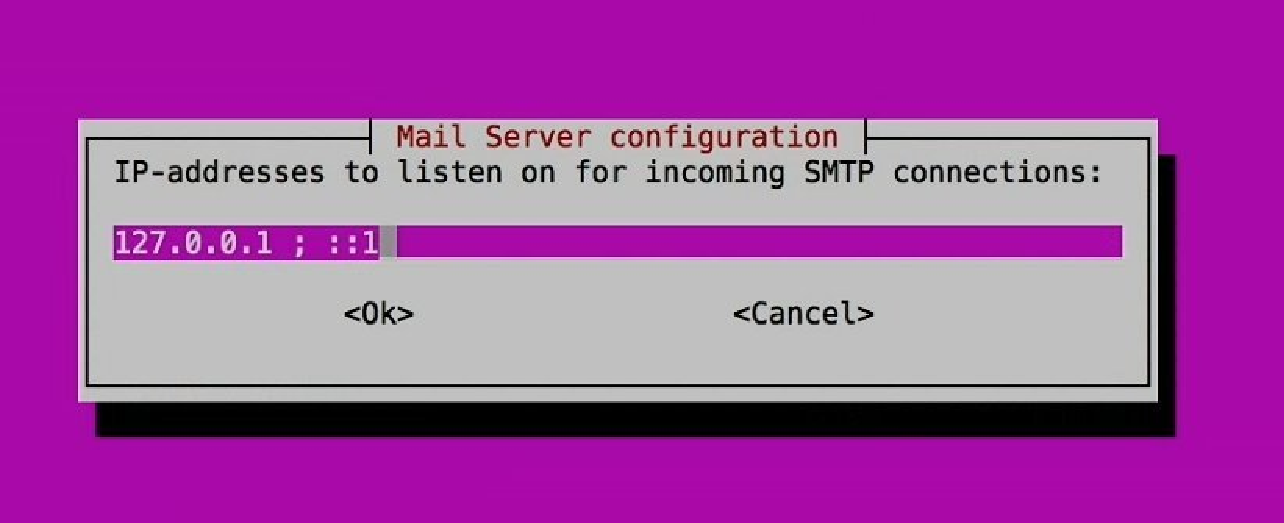
\includegraphics[width=.9\textwidth ,height=.35\textwidth]{Pic/EXIM4}
    \caption{ تنظیمات نرمافزار 
        \lr{ Exim}
        \lr{"Mail Server"}   
    }
    \label{MAIL-SERVER-EXIM4}
\end{figure}

این مرحله را نیز با تایید آن و بدون تغییر مقدار وارد شده به شکل پیش‌فرض، رها خواهیم کرد و با زدن دکمه اینتر بر روی گزینه تایید «OK» کادر را بسته و  وارد مرحله بعد خواهیم شد. \ref{MAIL-SERVER-EXIM5}

\begin{figure}
    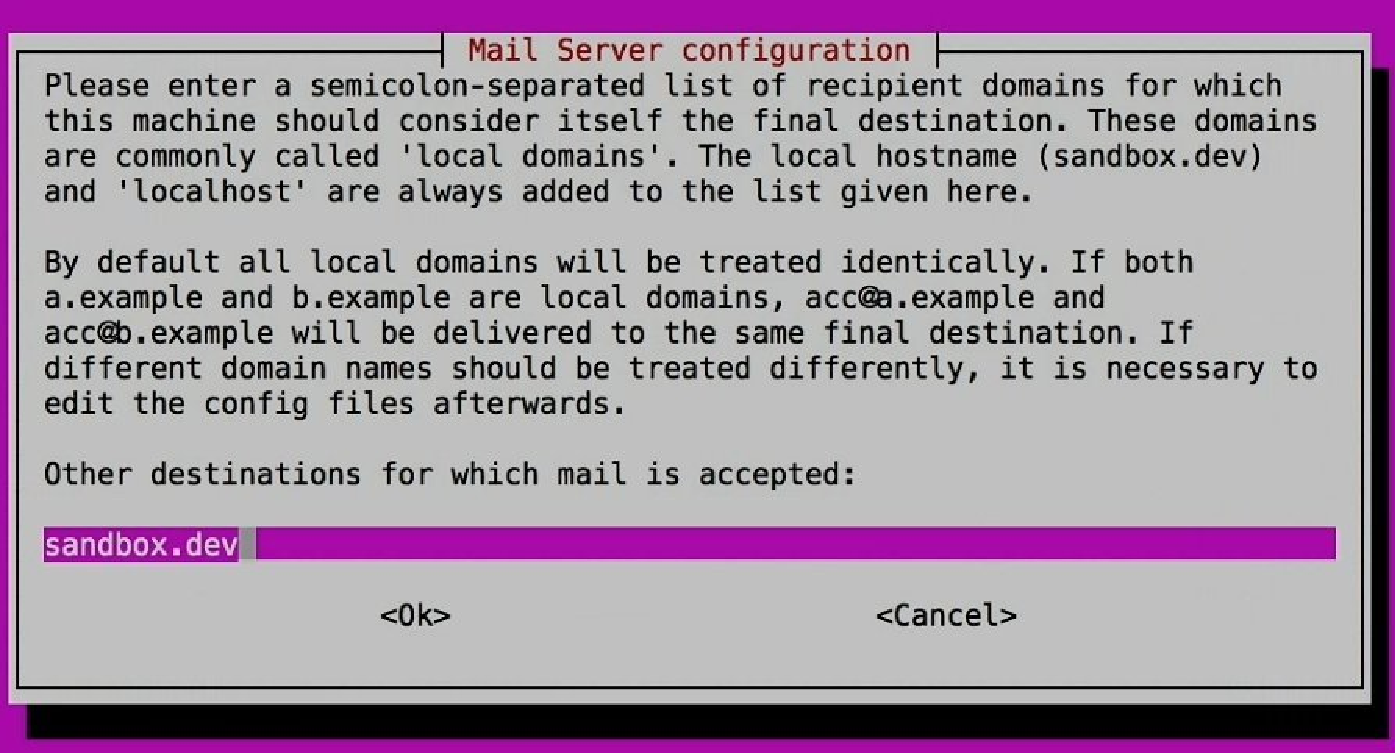
\includegraphics[width=.9\textwidth ,height=.45\textwidth]{Pic/EXIM5}
    \caption{ تنظیمات نرمافزار 
        \lr{ Exim}
        \lr{"Mail Server"}   
    }
    \label{MAIL-SERVER-EXIM5}
\end{figure}
در مرحله بعدی نیز چیزی را وارد نکرده و کادر را خالی رها می‌کنیم.
\ref{MAIL-SERVER-EXIM6}
\begin{figure}
    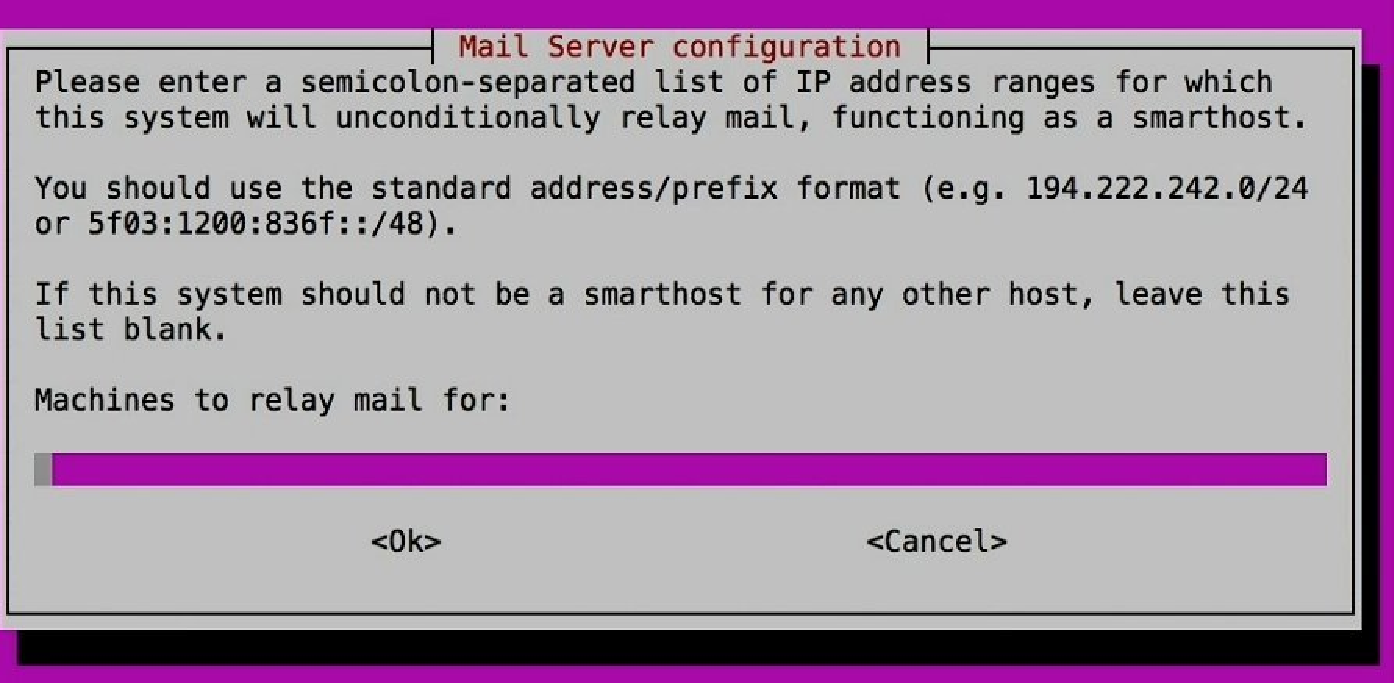
\includegraphics[width=.9\textwidth ,height=.45\textwidth]{Pic/EXIM6}
    \caption{ تنظیمات نرمافزار 
        \lr{ Exim}
        \lr{"Mail RELAAY"}   
    }
    \label{MAIL-SERVER-EXIM6}
\end{figure}
در مرحله بعدی باید آدرس سرور اس‌ام‌تی‌پی را وارد کنید. در این کادر باید آدرس سرور جی‌میل را وارد کنید که به صورتی که در تصویر مشاهده می‌شود آن را وارد می‌کنیم.
\ref{MAIL-SERVER-EXIM7}
\begin{figure}
    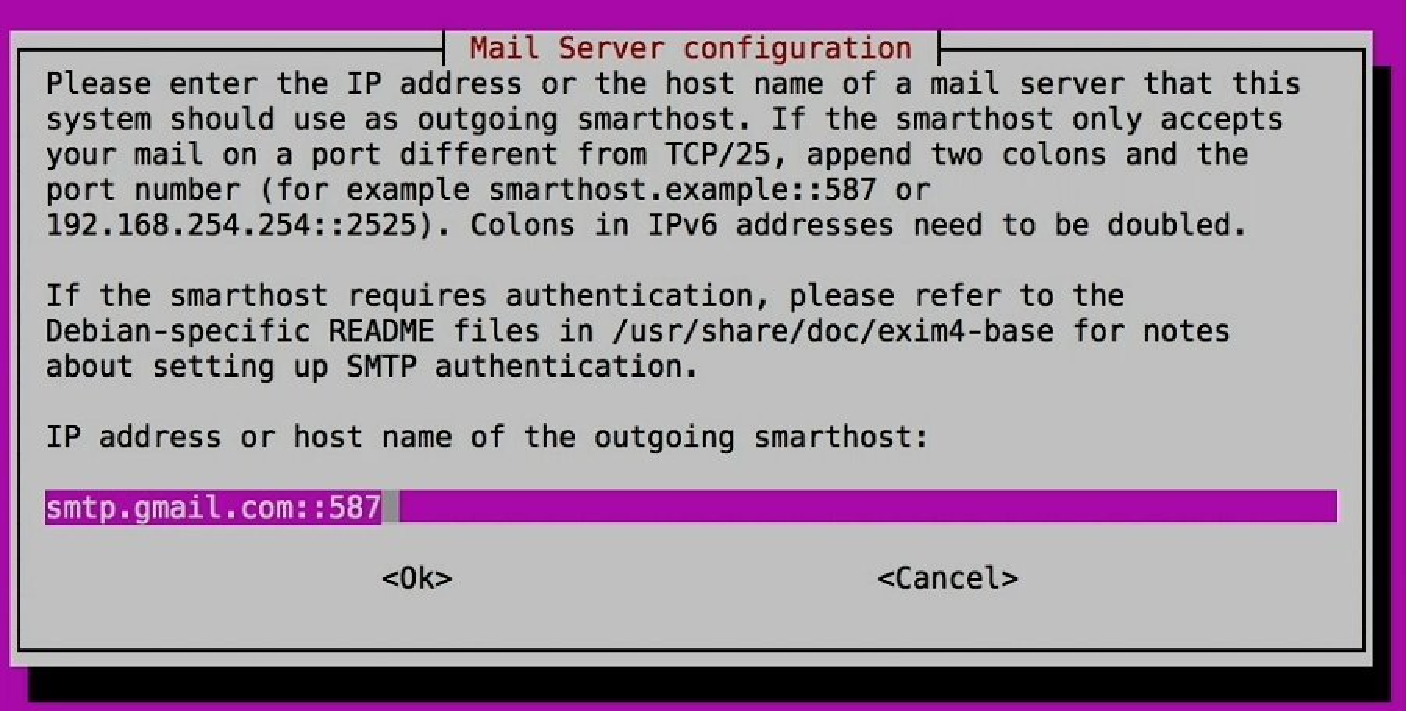
\includegraphics[width=.9\textwidth ,height=.45\textwidth]{Pic/EXIM7}
    \caption{ تنظیمات نرمافزار 
        \lr{ Exim}
        \lr{"Mail SMTP"}   
    }
    \label{MAIL-SERVER-EXIM7}
\end{figure}
در پیغام نمایش داده شده نیز بر روی نه «No» کلید اینتر را فشار می‌دهیم. در صورت اینکه بخواهید نام رایانامه محلی در پیام ارسالی دیده نشود، باید گزینه بله «Yes» را انتخاب کنید. \ref{MAIL-SERVER-EXIM8}

\begin{figure}
    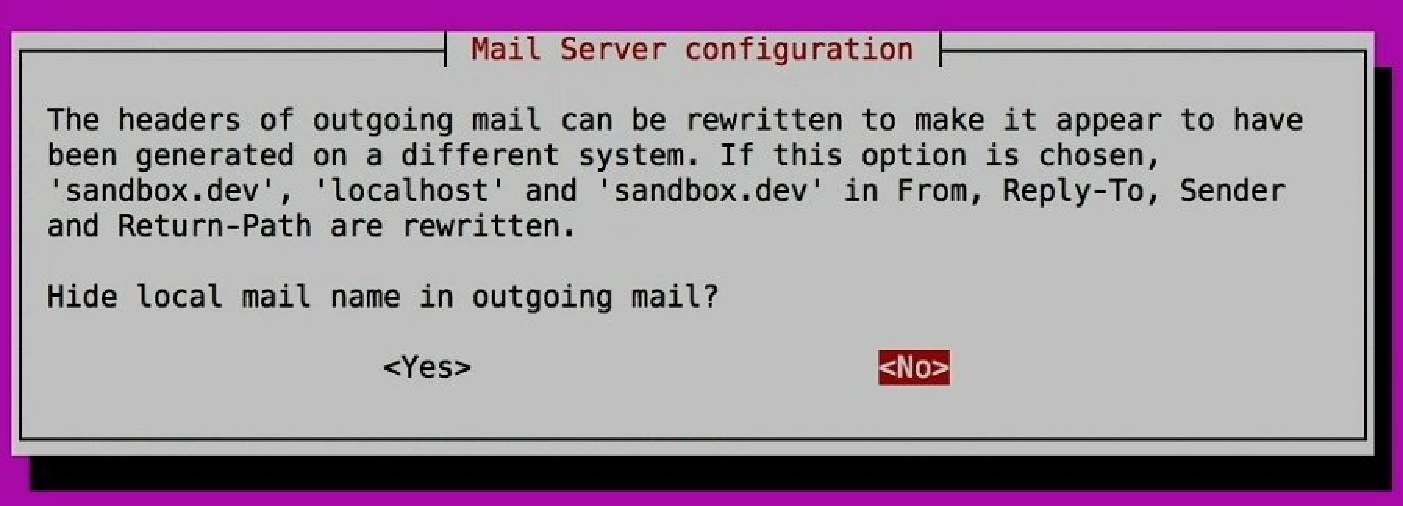
\includegraphics[width=.9\textwidth ,height=.35\textwidth]{Pic/EXIM8}
    \caption{ تنظیمات نرمافزار 
        \lr{ Exim}
        \lr{"Outgoing Mail"}   
    }
    \label{MAIL-SERVER-EXIM8}
\end{figure}
کادر نمایش داده شده در این مرحله را نیز تایید کرده تا به مراحل بعدی برویم.
 \ref{MAIL-SERVER-EXIM9}
\begin{figure}
    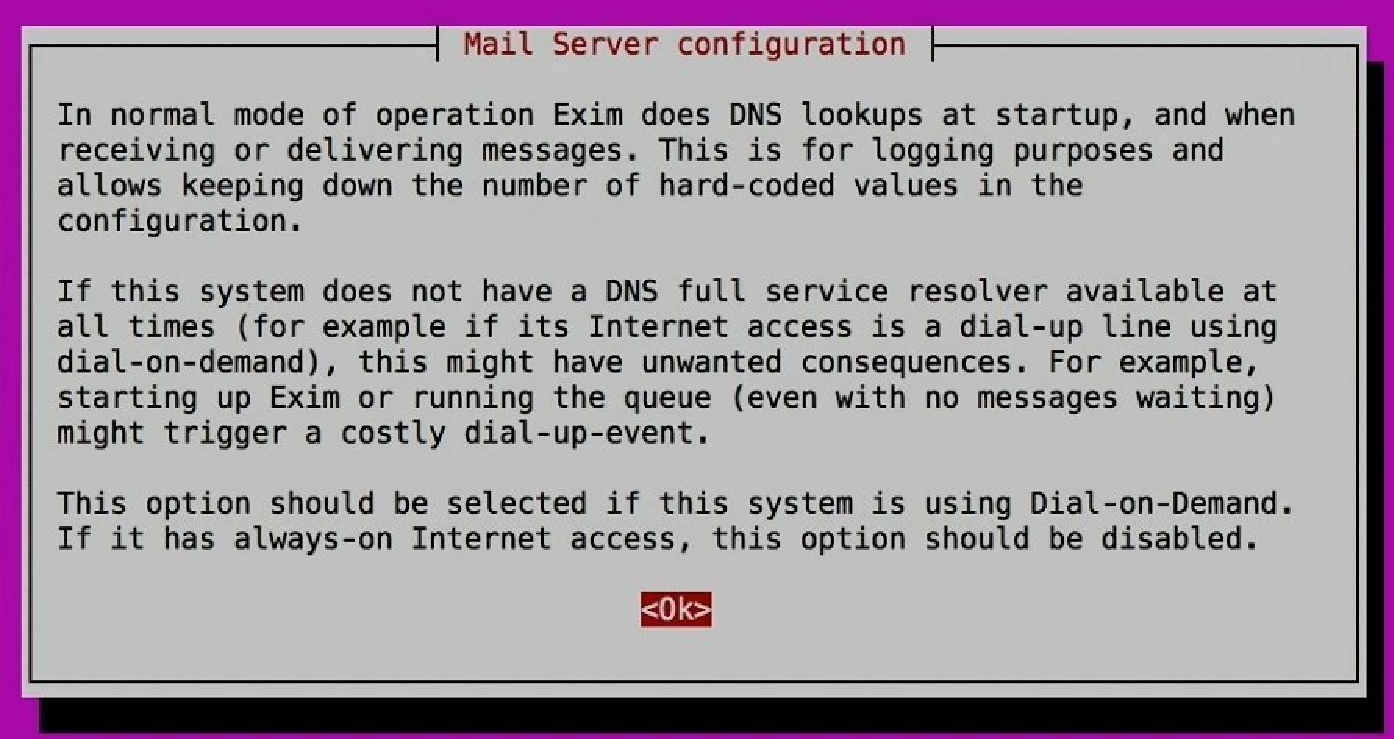
\includegraphics[width=.9\textwidth ,height=.50\textwidth]{Pic/EXIM9}
    \caption{ تنظیمات نرمافزار 
        \lr{ Exim}
        \lr{"Setup finished"}   
    }
    \label{MAIL-SERVER-EXIM9}
\end{figure}
سپس به دلیل  عدم تغییر گزینه‌ها، تصاویر دیگر مراحل را درج نکرده و پیشنهاد می‌شود که تا آخرین مراحل همه چیز را به صورت پیش‌فرض تایید کنید تا کادرهای نمایش داده و مراحل تنظیم به پایان برسد. حال با اتمام تمامی مراحل بالا باید به تنظیمات نرم‌افزار رفته و نام‌کاربری و رمز عبور خود را در آن وارد کنید. این نرم‌افزار نیز برای دسترسی به حساب کاربری شما نیاز به نوشتن نام کاربری و رمز‌عبور دارد که برای نوشتن این موارد، دستور زیر را در خط فرمان اجرا می‌شود.
\newline
\begin{latin}  
    \lstinputlisting[numbers=right,language=SH, framexleftmargin=5mm, frame=shadowbox,rulesepcolor=\color{Black}]{Code/exin-install3.sh}
\end{latin}
سپس خط زیر را به پایان فایل اضافه کنید. مقادیری مثل آدرس رایانامه و گذرواژه در دستور زیر را نیز با گذرواژه و رایانامه مورد نظر خود تعویض کنید، در این دستور می‌توانید گذرواژه خود را وارد کنید. دقت داشته باشید که اگر این فایل به دست فردی بیفتد، گذرواژه شما در اختیار آن فرد قرار خواهد گرفت.
\newline
\begin{latin}  
    \lstinputlisting[numbers=right,language=SH, framexleftmargin=5mm, frame=shadowbox,rulesepcolor=\color{Purple}]{Code/exin-install4.sh}
\end{latin}
بعد از انجام مراحل بالا و نوشتن مقادیر بالا در انتهای فایل مذکور، خواهید توانست با استفاده از خط فرمان برای فرد دیگری پیغامی را ارسال کنید. در این پیغام نمی‌توان از عناصر اچ‌تی‌ام‌ال استفاده کرد. بعد از نوشتن عنوان پیغام و سپس نوشتن بدنه پیغام و برای ارسال می‌بایست از کلید‌های 
\path{«CTRL + D»}
 استفاده کرد تا پیغام پایان یافته و برای گیرنده مشخص شده در دستور، ارسال شود.
\newline
\begin{latin}  
    \lstinputlisting[numbers=right,language=SH, framexleftmargin=5mm, frame=shadowbox,rulesepcolor=\color{Black}]{Code/exin-install5.sh}
\end{latin}
بعد از این کار اگر وارد حساب کاربری خود در پایگاه اینترنتی جی‌میل شوید، با پیغام نوشته شده در دستور مذکور، مواجه خواهید شد که به این معناست، تنظیمات به درستی انجام شده است. اگر پیغام ارسال نشد مجددا تنظیمات را از نوع و با دقت بیشتری انجام دهید. مثلا شاید آدرس اس‌ام‌تی‌پی را اشتباه وارد کرده‌اید.
\begin{figure}
    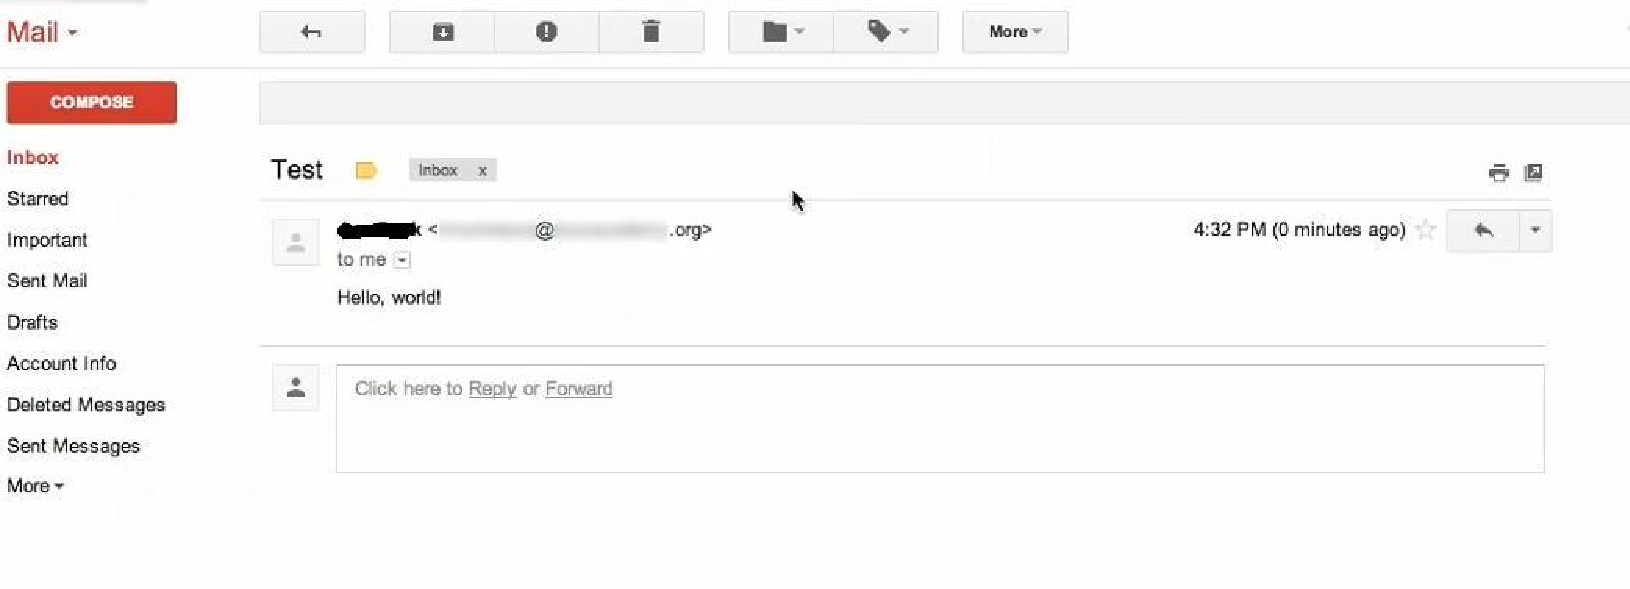
\includegraphics[width=.9\textwidth ,height=.40\textwidth]{Pic/GMAIL}
    \caption{ دریافت رایانامه از  
        \lr{ Exim}
        از
        \lr{"GMail"}   
    }
    \label{EMAIL-FROM-EXIM}
\end{figure}
در این مطلب، نحوه تنظیم پی‌اچ‌پی و برخی تنظیمات آن را آموزش داده و سپس با تنظیم مای‌اس‌کیوال و اتصال به آن توسط ابزار گرافیکی توسعه داده شده توسط اوراکل، نرم‌افزار مای‌اس‌کیوال ورک‌برنچ، این پایگاه داده متن‌باز را نیز بررسی کردیم. در ادامه نیز نحوه ارسال رایانامه توسط ابزار اگزیم۴ را نیز آموخته و توانستیم یک رایانامه متنی را  توسط خط فرمان ارسال کنیم. بعد از قسمت سوم این آموزش نحوه نصب و تنظیم اوبونتو به صورت سندباکس، شما قادر خواهید بود تا کد‌های بهره‌مند از بانک اطلاعاتی مای‌اس‌کیوال و پی‌اچ‌پی  یا حتی اس‌کیولایت خود را به راحتی و بی هیچ مشکلی اجرا نمایید. در قسمت بعدی یعنی قسمت آخر و چهارم این آموزش، معرفی و نصب ابزارهای تحت وب، مانند پی‌اچ‌پی مای‌ادمین و همچنین ابزارهای مدیر محتوای متن‌باز دروپال و وردپرس و ابزارهای تحت‌وب دیگر را نیز بررسی خواهیم کرد.

در آخر لازم به ذکر است که اگر قصد داشته باشید که موارد گفته شده در این آموزش را به صورت مجزا  و در یک سرور حقیقی نیز اجرا کنید، با کمی تغییر در کدهای معرفی شده و تنظیمات صورت گرفته خواهید توانست سرور واقعی خود را راه‌اندازی کنید. برای این کار کافی است از یک رایانه قدیمی و یا حتی رزبری‌پای استفاده کنید و تصویر اوبونتو سرور را بر روی آن نصب کنید، سپس با اتصال آن شبکه به یک شبکه محلی خواهید توانست با انتقال درگاه در رایانه مورد نظر، به آن سرور به صورت اس‌اس‌اچ متصل شوید و با طی مراحل مشابه این مقاله آموزشی ولی با کمی تغییرات، سرور محلی خود را ایجاد نمایید. چنین کاری باعث می‌شود تا شما برای مدیریت یک سرور واقعی در محیط اینترنت نیز، آمادگی لازم و کافی را داشته باشید.